\documentclass[11pt]{article}
\usepackage[margin=1in]{geometry}
\usepackage{graphicx}
\usepackage{amsmath}
\usepackage{booktabs}

\title{A Finite Intercept Correction Calculation}
\author{Anonymous}
\date{}

\begin{document}
\maketitle

\begin{abstract}
This teaching note follows a fixed predictor through residual calculation, intercept correction, and evaluation on five synthetic observations. For targets $y=2x+3$, the predictor $2x$ has residual $3$ at every supplied input. Adding the mean residual gives exact agreement on these observations. Three recorded corrections connect mean absolute error with mean squared error, while a dependency diagram identifies the observations used at each step. The instructional objective is to distinguish computing a correction from interpreting the error measured on the observations that determine it.
\end{abstract}

\section{Introduction}

For students beginning regression, an explicit numerical example can connect prediction, residuals, adjustment, and error measurement. This note presents an established least-squares intercept calculation as a worked teaching example. Its contribution is instructional: all inputs and recorded outputs are stated, the arithmetic is linked to an error table and plot, and a diagram traces the reuse of observations.

The example keeps the slope fixed so that readers can follow a single estimated quantity, the additive correction. Three learning objectives organize the presentation: compute the mean residual, explain the different responses of absolute and squared error to partial correction, and identify which observations determine and assess the adjustment. The reported errors are checks of the supplied finite calculation.

\section{Related Work}

Residual examination connects numerical discrepancies with graphical assessment of fitted analyses \cite{Anscombe1963ExaminationAnalysis}. Here, identical residuals make that connection directly inspectable. Eisenhauer discusses regression through the origin and its evaluative statistics \cite{Eisenhauer2003RegressionThrough}; the present baseline also has zero intercept, with its slope supplied rather than estimated. Shmueli distinguishes explanatory and predictive modeling goals \cite{Shmueli2010ExplainOr}. That distinction motivates labeling the present comparison by its assessment observations. These references frame the teaching objectives; the calculation uses only the stated predictor and targets.

\section{Method}

\subsection{Finite Inputs and Fixed Predictor}

The five observations and baseline predictions, in their supplied order, are
\[
\begin{aligned}
x&=(-2,-1,0,1,2),\\
y&=(-1,1,3,5,7),\\
\widehat{y}^{(0)}=2x&=(-4,-2,0,2,4).
\end{aligned}
\]
Subtracting baseline predictions from targets gives
\[
r_i=y_i-2x_i,\qquad
(r_1,r_2,r_3,r_4,r_5)=(3,3,3,3,3).
\]
Thus, every baseline prediction is below its target by the same amount. Both the slope and the observations are fixed inputs to this calculation.

\subsection{Mean-Residual Correction and Data Dependencies}

The estimated additive correction is
\[
b=\bar r=\frac{1}{5}\sum_{i=1}^{5}r_i
=\frac{3+3+3+3+3}{5}=3.
\]
Substitution gives the corrected predictions
\[
\widehat{y}^{(b)}_i=2x_i+b=2x_i+3=y_i.
\]
For these residuals, the least-squares role of their mean follows by expansion:
\[
\begin{aligned}
\frac{1}{5}\sum_{i=1}^{5}(r_i-b)^2
&=\frac{1}{5}\sum_{i=1}^{5}(r_i-\bar r)^2
 +(b-\bar r)^2\\
&=(b-3)^2.
\end{aligned}
\]
The cross term vanishes because the centered residuals sum to zero. The first term is zero because all five residuals equal their mean; the second becomes zero at $b=3$. This separates choosing the least-squares constant from the identical-residual property responsible for exact agreement.

Figure~\ref{fig:residual_workflow} traces the computation. Targets and baseline predictions determine residuals; residuals determine $b$; corrected predictions are compared with the original targets. Reading the dashed arrow alongside the equations identifies the reported error as an in-sample check.

\begin{figure}[!htbp]
\centering
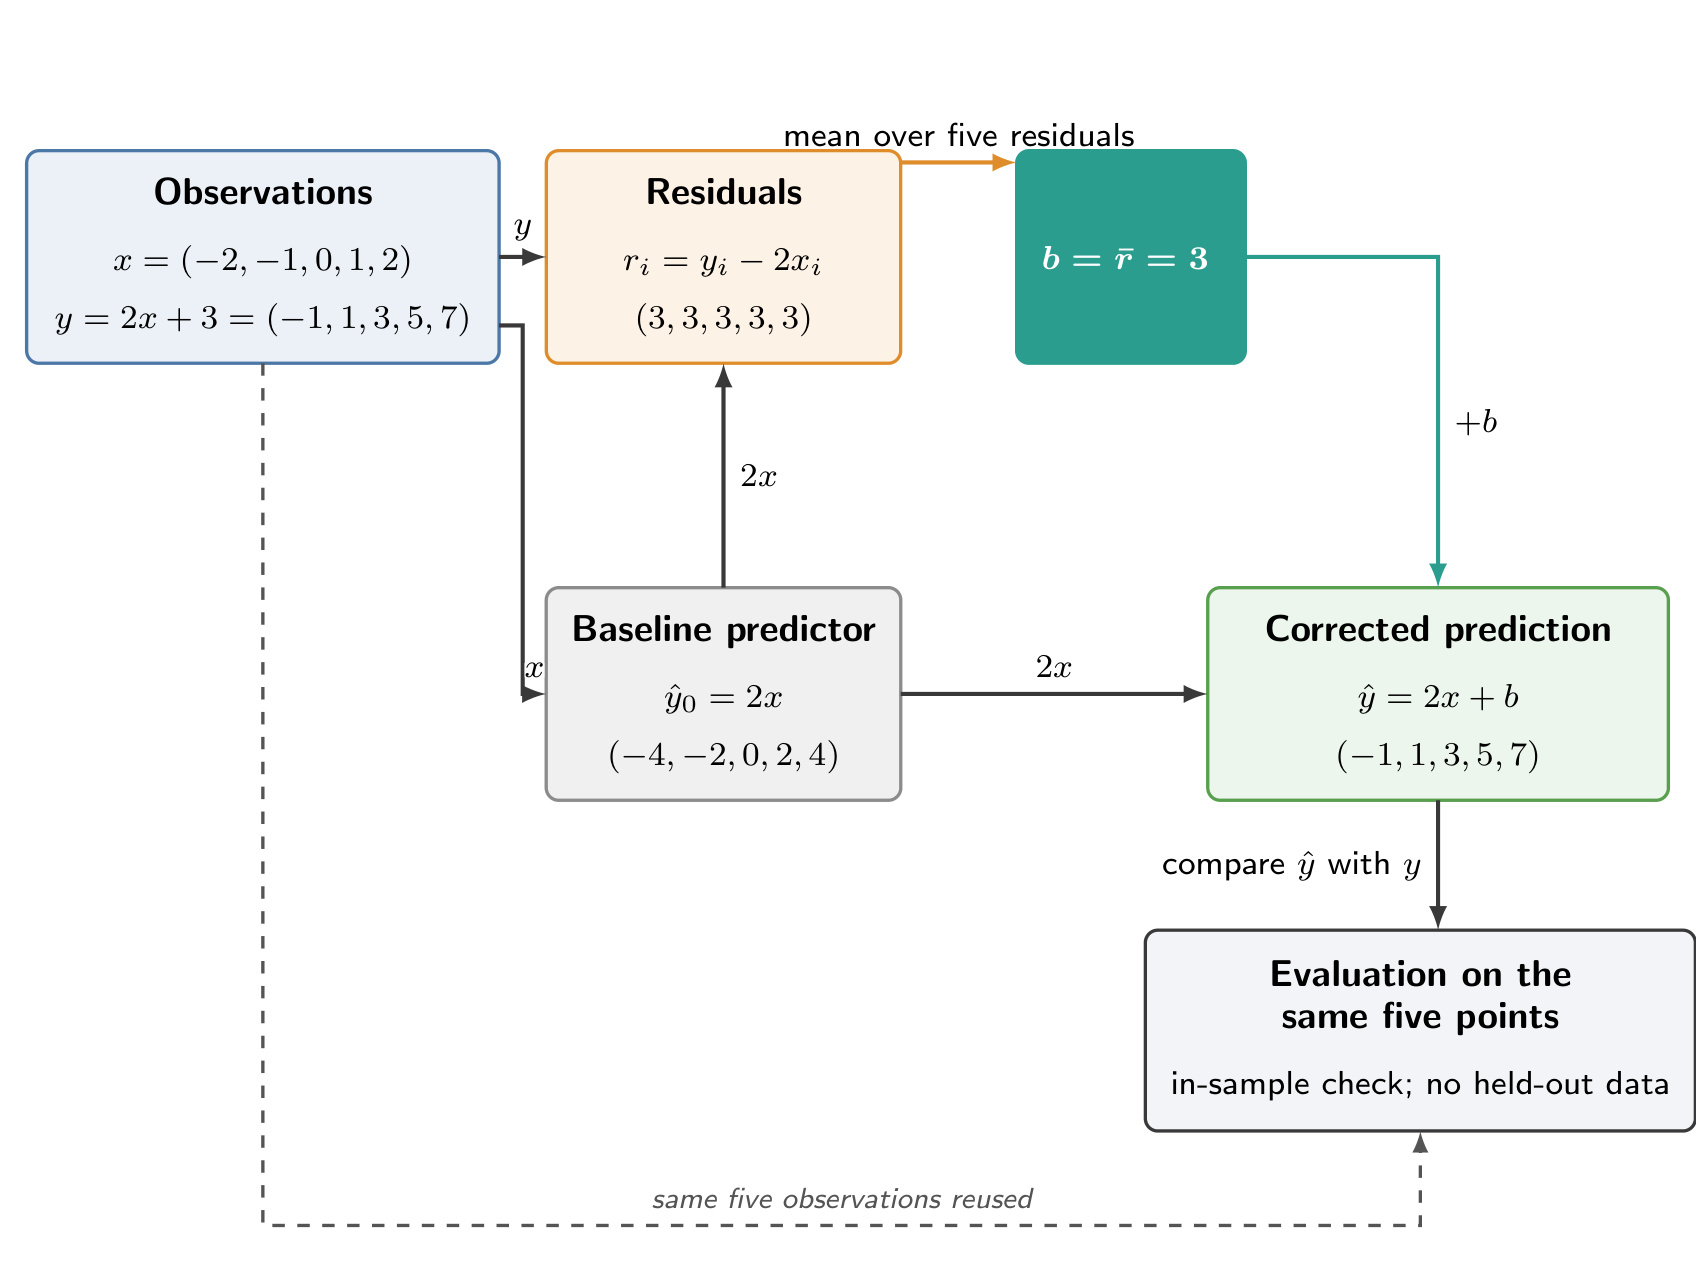
\includegraphics[width=\linewidth]{figures/fig_residual_workflow.jpg}
\caption{Residual correction and assessment on the same five observations. The solid arrows trace the calculation of $b=3$ and corrected predictions. The dashed arrow identifies the original observations reused for evaluation.}
\label{fig:residual_workflow}
\end{figure}

\section{Experiments}

\subsection{Recorded Calculation and Error Definitions}

The recorded computation is one deterministic calculation in base R. For an added scalar $b$, define
\[
e_i(b)=y_i-(2x_i+b),
\]
with errors
\[
\operatorname{MAE}(b)=\frac{1}{5}\sum_{i=1}^{5}|e_i(b)|,
\qquad
\operatorname{MSE}(b)=\frac{1}{5}\sum_{i=1}^{5}e_i(b)^2.
\]
The three recorded settings are $b=0$, $1.5$, and $3$. They represent the baseline, a supplied partial correction, and the observed mean-residual correction. Each setting is evaluated against the same five targets.

The intermediate setting has a specific instructional purpose: adding $1.5$ removes half the baseline discrepancy. Its remaining residual is $1.5$ at every point, so MAE halves while MSE becomes one quarter of its baseline value. This contrasts the linear and squared penalties using the same residual pattern. The setting is a comparison value, rather than an iteration in an optimization procedure.

\subsection{Measured Errors and Visualization}

Table~\ref{tab:recorded_errors} contains all recorded error values. They can be checked directly from the supplied observations using
\[
e_i(b)=3-b,\qquad
\operatorname{MAE}(b)=|3-b|,\qquad
\operatorname{MSE}(b)=(3-b)^2.
\]
At $b=3$, all corrected predictions equal their recorded targets. Together, the table and residual decomposition explain both the progression of the errors and the exact endpoint.

\begin{table}[!htbp]
\centering
\caption{Recorded errors, evaluated on the five observations used to calculate the mean-residual correction.}
\label{tab:recorded_errors}
\begin{tabular}{rrr}
\toprule
Added $b$ & Mean absolute error & Mean squared error \\
\midrule
0   & 3   & 9    \\
1.5 & 1.5 & 2.25 \\
3   & 0   & 0    \\
\bottomrule
\end{tabular}
\end{table}

Figure~\ref{fig:intercept_error} displays precisely these three recorded MSE pairs. Its discrete markers distinguish the measured settings from the algebraic identity used to explain them. A classroom reading can proceed from each correction to its residual, then to its absolute and squared errors, and finally back to the observation-reuse arrow in Figure~\ref{fig:residual_workflow}.

\begin{figure}[!htbp]
\centering
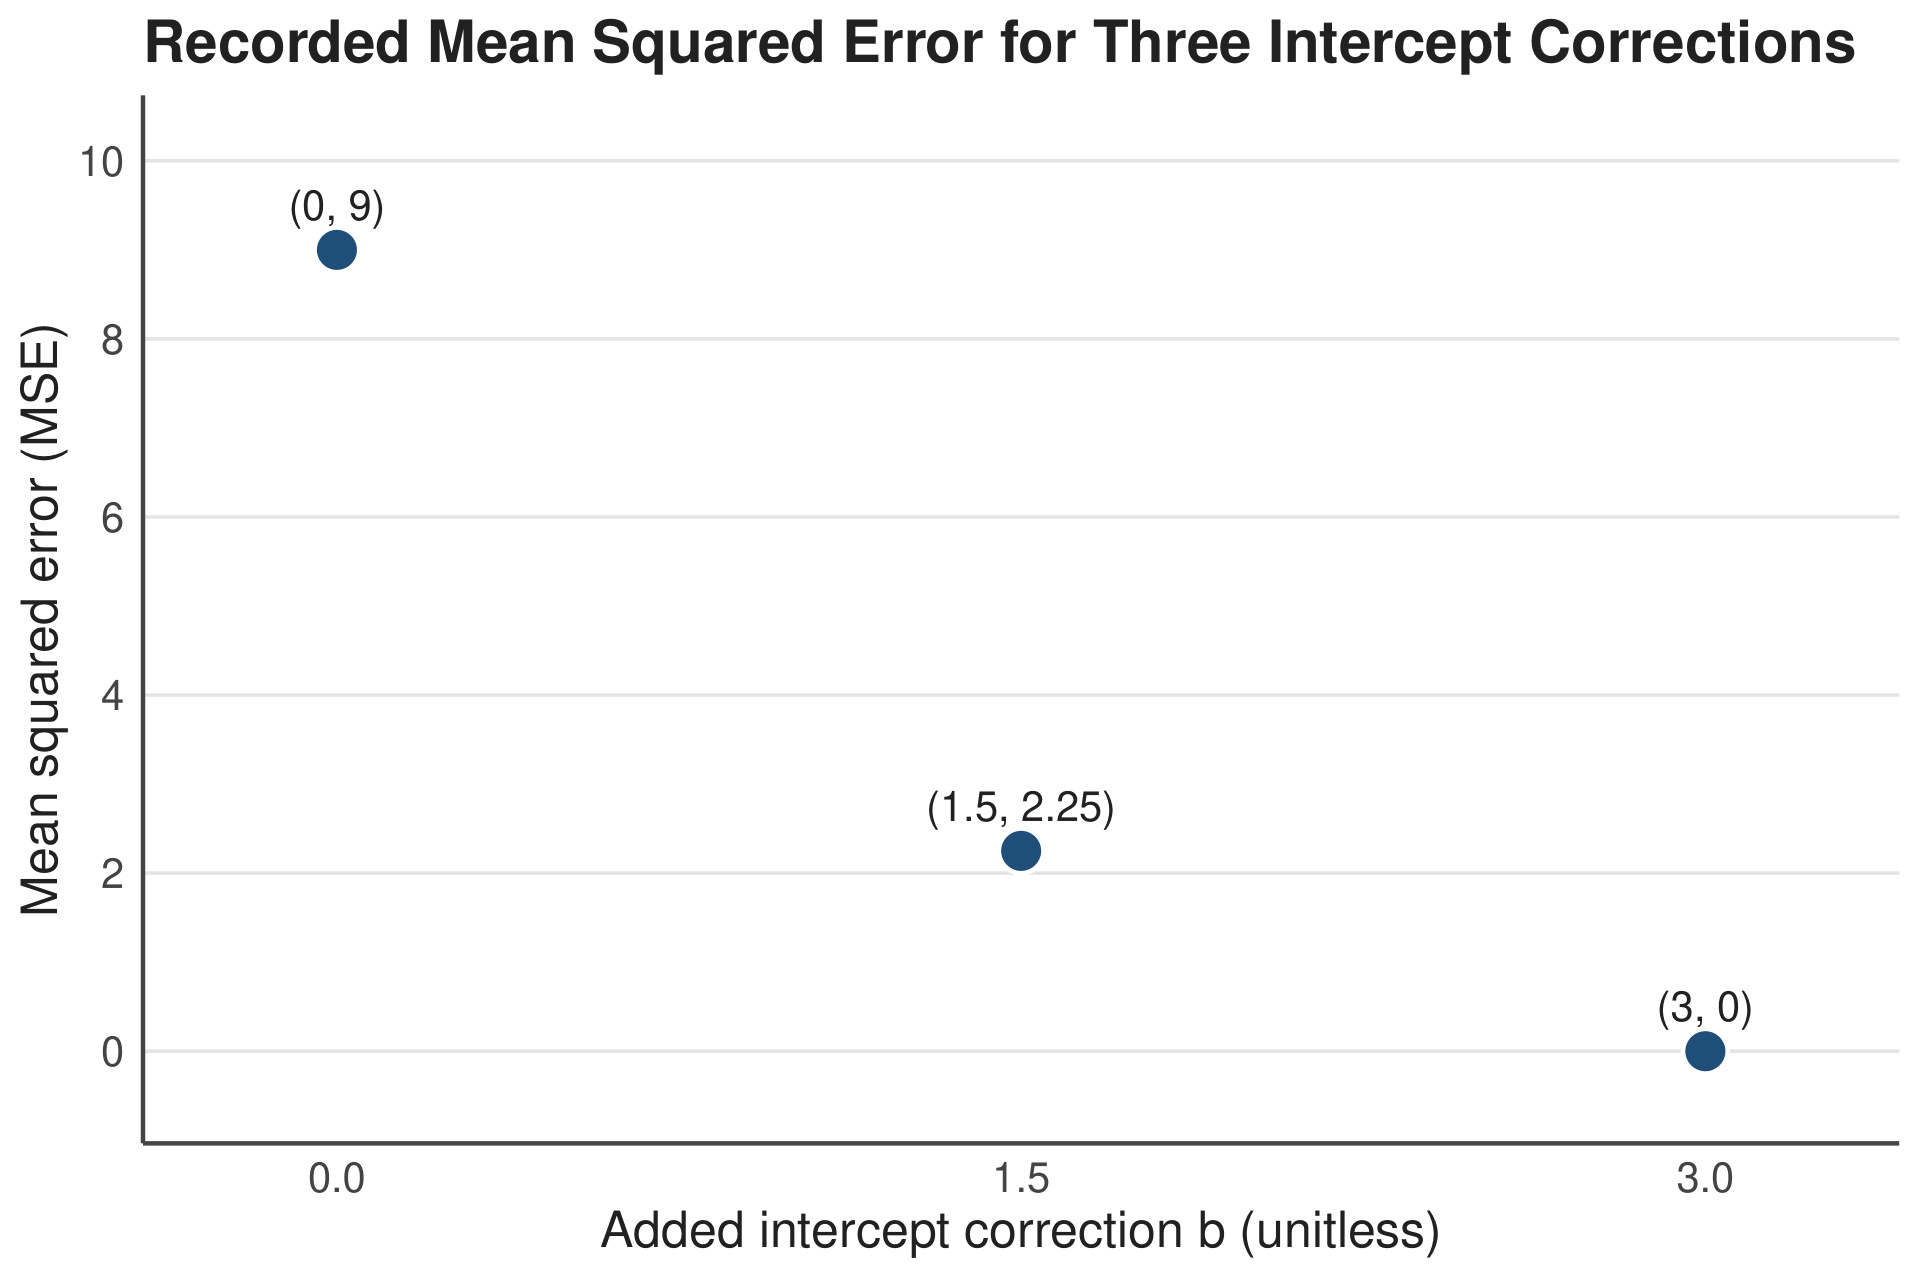
\includegraphics[width=\linewidth]{figures/fig_intercept_error.jpg}
\caption{Recorded pairs $(b,\operatorname{MSE})=(0,9)$, $(1.5,2.25)$, and $(3,0)$. Each label identifies an in-sample error calculated from the same five targets.}
\label{fig:intercept_error}
\end{figure}

\section{Conclusion}

Adding the observed mean residual, $3$, to the fixed predictor $2x$ exactly corrects its shared discrepancy on the five supplied observations. The partial correction connects absolute and squared error, while the residual decomposition explains the zero endpoint. The teaching example combines an inspectable calculation with an explicit account of which observations determine and assess the correction.


\begin{thebibliography}{9}

\bibitem{Anscombe1963ExaminationAnalysis}
Francis John Anscombe and John W. Tukey.
\newblock The Examination and Analysis of Residuals.
\newblock \emph{Technometrics}, 1963.

\bibitem{Eisenhauer2003RegressionThrough}
Joseph G. Eisenhauer.
\newblock Regression through the Origin.
\newblock \emph{Teaching Statistics}, 2003.

\bibitem{Shmueli2010ExplainOr}
Galit Shmueli.
\newblock To Explain or to Predict?
\newblock \emph{Statistical Science}, 2010.

\end{thebibliography}

% PAPER_ORCHESTRA_PROVENANCE_BEGIN
\clearpage
\section*{Figure source provenance}
The files below are the exact sources that produced the embedded figure previews. Paths are relative to this manuscript's source directory. The accompanying \texttt{figure\char95{}provenance.json} records all artifact checksums.\par
\medskip\noindent\textbf{Figure~\ref{fig:intercept_error} (\texttt{fig\char95{}intercept\char95{}error.jpg}).}\par
\noindent R/ggplot2 source: \texttt{figure\char95{}code/\allowbreak{}fig\char95{}intercept\char95{}error/\allowbreak{}source.R}.\par
\noindent Source SHA256: \texttt{34ba57e5\allowbreak{}6adf6b78\allowbreak{}4bfabe24\allowbreak{}299ef6d2\allowbreak{}5ce74051\allowbreak{}70d96d8c\allowbreak{}09ada698\allowbreak{}97622aee}.\par
\noindent Rendering metadata: \texttt{figure\char95{}code/\allowbreak{}fig\char95{}intercept\char95{}error/\allowbreak{}render.json}.\par
\noindent Exact export wrapper: \texttt{figure\char95{}code/\allowbreak{}fig\char95{}intercept\char95{}error/\allowbreak{}worker.R}.\par
\noindent Wrapper SHA256: \texttt{1aedad4b\allowbreak{}1547d4b2\allowbreak{}d394cbb0\allowbreak{}239655d3\allowbreak{}667d453d\allowbreak{}d1fd0eca\allowbreak{}3e77c037\allowbreak{}e6d34892}.\par
\noindent Rendering metadata: \texttt{figure\char95{}code/\allowbreak{}fig\char95{}intercept\char95{}error/\allowbreak{}sessionInfo.txt}.\par
\medskip\noindent\textbf{Figure~\ref{fig:residual_workflow} (\texttt{fig\char95{}residual\char95{}workflow.jpg}).}\par
\noindent LaTeX/TikZ source: \texttt{figure\char95{}code/\allowbreak{}fig\char95{}residual\char95{}workflow/\allowbreak{}source.tex}.\par
\noindent Source SHA256: \texttt{e1de201d\allowbreak{}70c4a996\allowbreak{}77d8214a\allowbreak{}b33a2f9c\allowbreak{}6815b281\allowbreak{}a8c5bf20\allowbreak{}97e46cce\allowbreak{}5855da92}.\par
\noindent Rendering metadata: \texttt{figure\char95{}code/\allowbreak{}fig\char95{}residual\char95{}workflow/\allowbreak{}render.json}.\par
% PAPER_ORCHESTRA_PROVENANCE_END
\end{document}